% Options for packages loaded elsewhere
% Options for packages loaded elsewhere
\PassOptionsToPackage{unicode}{hyperref}
\PassOptionsToPackage{hyphens}{url}
\PassOptionsToPackage{dvipsnames,svgnames,x11names}{xcolor}
%
\documentclass[
  letterpaper,
  DIV=11,
  numbers=noendperiod]{scrartcl}
\usepackage{xcolor}
\usepackage{amsmath,amssymb}
\setcounter{secnumdepth}{-\maxdimen} % remove section numbering
\usepackage{iftex}
\ifPDFTeX
  \usepackage[T1]{fontenc}
  \usepackage[utf8]{inputenc}
  \usepackage{textcomp} % provide euro and other symbols
\else % if luatex or xetex
  \usepackage{unicode-math} % this also loads fontspec
  \defaultfontfeatures{Scale=MatchLowercase}
  \defaultfontfeatures[\rmfamily]{Ligatures=TeX,Scale=1}
\fi
\usepackage{lmodern}
\ifPDFTeX\else
  % xetex/luatex font selection
\fi
% Use upquote if available, for straight quotes in verbatim environments
\IfFileExists{upquote.sty}{\usepackage{upquote}}{}
\IfFileExists{microtype.sty}{% use microtype if available
  \usepackage[]{microtype}
  \UseMicrotypeSet[protrusion]{basicmath} % disable protrusion for tt fonts
}{}
\makeatletter
\@ifundefined{KOMAClassName}{% if non-KOMA class
  \IfFileExists{parskip.sty}{%
    \usepackage{parskip}
  }{% else
    \setlength{\parindent}{0pt}
    \setlength{\parskip}{6pt plus 2pt minus 1pt}}
}{% if KOMA class
  \KOMAoptions{parskip=half}}
\makeatother
% Make \paragraph and \subparagraph free-standing
\makeatletter
\ifx\paragraph\undefined\else
  \let\oldparagraph\paragraph
  \renewcommand{\paragraph}{
    \@ifstar
      \xxxParagraphStar
      \xxxParagraphNoStar
  }
  \newcommand{\xxxParagraphStar}[1]{\oldparagraph*{#1}\mbox{}}
  \newcommand{\xxxParagraphNoStar}[1]{\oldparagraph{#1}\mbox{}}
\fi
\ifx\subparagraph\undefined\else
  \let\oldsubparagraph\subparagraph
  \renewcommand{\subparagraph}{
    \@ifstar
      \xxxSubParagraphStar
      \xxxSubParagraphNoStar
  }
  \newcommand{\xxxSubParagraphStar}[1]{\oldsubparagraph*{#1}\mbox{}}
  \newcommand{\xxxSubParagraphNoStar}[1]{\oldsubparagraph{#1}\mbox{}}
\fi
\makeatother

\usepackage{color}
\usepackage{fancyvrb}
\newcommand{\VerbBar}{|}
\newcommand{\VERB}{\Verb[commandchars=\\\{\}]}
\DefineVerbatimEnvironment{Highlighting}{Verbatim}{commandchars=\\\{\}}
% Add ',fontsize=\small' for more characters per line
\usepackage{framed}
\definecolor{shadecolor}{RGB}{241,243,245}
\newenvironment{Shaded}{\begin{snugshade}}{\end{snugshade}}
\newcommand{\AlertTok}[1]{\textcolor[rgb]{0.68,0.00,0.00}{#1}}
\newcommand{\AnnotationTok}[1]{\textcolor[rgb]{0.37,0.37,0.37}{#1}}
\newcommand{\AttributeTok}[1]{\textcolor[rgb]{0.40,0.45,0.13}{#1}}
\newcommand{\BaseNTok}[1]{\textcolor[rgb]{0.68,0.00,0.00}{#1}}
\newcommand{\BuiltInTok}[1]{\textcolor[rgb]{0.00,0.23,0.31}{#1}}
\newcommand{\CharTok}[1]{\textcolor[rgb]{0.13,0.47,0.30}{#1}}
\newcommand{\CommentTok}[1]{\textcolor[rgb]{0.37,0.37,0.37}{#1}}
\newcommand{\CommentVarTok}[1]{\textcolor[rgb]{0.37,0.37,0.37}{\textit{#1}}}
\newcommand{\ConstantTok}[1]{\textcolor[rgb]{0.56,0.35,0.01}{#1}}
\newcommand{\ControlFlowTok}[1]{\textcolor[rgb]{0.00,0.23,0.31}{\textbf{#1}}}
\newcommand{\DataTypeTok}[1]{\textcolor[rgb]{0.68,0.00,0.00}{#1}}
\newcommand{\DecValTok}[1]{\textcolor[rgb]{0.68,0.00,0.00}{#1}}
\newcommand{\DocumentationTok}[1]{\textcolor[rgb]{0.37,0.37,0.37}{\textit{#1}}}
\newcommand{\ErrorTok}[1]{\textcolor[rgb]{0.68,0.00,0.00}{#1}}
\newcommand{\ExtensionTok}[1]{\textcolor[rgb]{0.00,0.23,0.31}{#1}}
\newcommand{\FloatTok}[1]{\textcolor[rgb]{0.68,0.00,0.00}{#1}}
\newcommand{\FunctionTok}[1]{\textcolor[rgb]{0.28,0.35,0.67}{#1}}
\newcommand{\ImportTok}[1]{\textcolor[rgb]{0.00,0.46,0.62}{#1}}
\newcommand{\InformationTok}[1]{\textcolor[rgb]{0.37,0.37,0.37}{#1}}
\newcommand{\KeywordTok}[1]{\textcolor[rgb]{0.00,0.23,0.31}{\textbf{#1}}}
\newcommand{\NormalTok}[1]{\textcolor[rgb]{0.00,0.23,0.31}{#1}}
\newcommand{\OperatorTok}[1]{\textcolor[rgb]{0.37,0.37,0.37}{#1}}
\newcommand{\OtherTok}[1]{\textcolor[rgb]{0.00,0.23,0.31}{#1}}
\newcommand{\PreprocessorTok}[1]{\textcolor[rgb]{0.68,0.00,0.00}{#1}}
\newcommand{\RegionMarkerTok}[1]{\textcolor[rgb]{0.00,0.23,0.31}{#1}}
\newcommand{\SpecialCharTok}[1]{\textcolor[rgb]{0.37,0.37,0.37}{#1}}
\newcommand{\SpecialStringTok}[1]{\textcolor[rgb]{0.13,0.47,0.30}{#1}}
\newcommand{\StringTok}[1]{\textcolor[rgb]{0.13,0.47,0.30}{#1}}
\newcommand{\VariableTok}[1]{\textcolor[rgb]{0.07,0.07,0.07}{#1}}
\newcommand{\VerbatimStringTok}[1]{\textcolor[rgb]{0.13,0.47,0.30}{#1}}
\newcommand{\WarningTok}[1]{\textcolor[rgb]{0.37,0.37,0.37}{\textit{#1}}}

\usepackage{longtable,booktabs,array}
\usepackage{calc} % for calculating minipage widths
% Correct order of tables after \paragraph or \subparagraph
\usepackage{etoolbox}
\makeatletter
\patchcmd\longtable{\par}{\if@noskipsec\mbox{}\fi\par}{}{}
\makeatother
% Allow footnotes in longtable head/foot
\IfFileExists{footnotehyper.sty}{\usepackage{footnotehyper}}{\usepackage{footnote}}
\makesavenoteenv{longtable}
\usepackage{graphicx}
\makeatletter
\newsavebox\pandoc@box
\newcommand*\pandocbounded[1]{% scales image to fit in text height/width
  \sbox\pandoc@box{#1}%
  \Gscale@div\@tempa{\textheight}{\dimexpr\ht\pandoc@box+\dp\pandoc@box\relax}%
  \Gscale@div\@tempb{\linewidth}{\wd\pandoc@box}%
  \ifdim\@tempb\p@<\@tempa\p@\let\@tempa\@tempb\fi% select the smaller of both
  \ifdim\@tempa\p@<\p@\scalebox{\@tempa}{\usebox\pandoc@box}%
  \else\usebox{\pandoc@box}%
  \fi%
}
% Set default figure placement to htbp
\def\fps@figure{htbp}
\makeatother





\setlength{\emergencystretch}{3em} % prevent overfull lines

\providecommand{\tightlist}{%
  \setlength{\itemsep}{0pt}\setlength{\parskip}{0pt}}



 


\usepackage{fvextra}
\DefineVerbatimEnvironment{Highlighting}{Verbatim}{breaklines,commandchars=\\\{\}}
\KOMAoption{captions}{tableheading}
\makeatletter
\@ifpackageloaded{tcolorbox}{}{\usepackage[skins,breakable]{tcolorbox}}
\@ifpackageloaded{fontawesome5}{}{\usepackage{fontawesome5}}
\definecolor{quarto-callout-color}{HTML}{909090}
\definecolor{quarto-callout-note-color}{HTML}{0758E5}
\definecolor{quarto-callout-important-color}{HTML}{CC1914}
\definecolor{quarto-callout-warning-color}{HTML}{EB9113}
\definecolor{quarto-callout-tip-color}{HTML}{00A047}
\definecolor{quarto-callout-caution-color}{HTML}{FC5300}
\definecolor{quarto-callout-color-frame}{HTML}{acacac}
\definecolor{quarto-callout-note-color-frame}{HTML}{4582ec}
\definecolor{quarto-callout-important-color-frame}{HTML}{d9534f}
\definecolor{quarto-callout-warning-color-frame}{HTML}{f0ad4e}
\definecolor{quarto-callout-tip-color-frame}{HTML}{02b875}
\definecolor{quarto-callout-caution-color-frame}{HTML}{fd7e14}
\makeatother
\makeatletter
\@ifpackageloaded{caption}{}{\usepackage{caption}}
\AtBeginDocument{%
\ifdefined\contentsname
  \renewcommand*\contentsname{Table of contents}
\else
  \newcommand\contentsname{Table of contents}
\fi
\ifdefined\listfigurename
  \renewcommand*\listfigurename{List of Figures}
\else
  \newcommand\listfigurename{List of Figures}
\fi
\ifdefined\listtablename
  \renewcommand*\listtablename{List of Tables}
\else
  \newcommand\listtablename{List of Tables}
\fi
\ifdefined\figurename
  \renewcommand*\figurename{Figure}
\else
  \newcommand\figurename{Figure}
\fi
\ifdefined\tablename
  \renewcommand*\tablename{Table}
\else
  \newcommand\tablename{Table}
\fi
}
\@ifpackageloaded{float}{}{\usepackage{float}}
\floatstyle{ruled}
\@ifundefined{c@chapter}{\newfloat{codelisting}{h}{lop}}{\newfloat{codelisting}{h}{lop}[chapter]}
\floatname{codelisting}{Listing}
\newcommand*\listoflistings{\listof{codelisting}{List of Listings}}
\makeatother
\makeatletter
\makeatother
\makeatletter
\@ifpackageloaded{caption}{}{\usepackage{caption}}
\@ifpackageloaded{subcaption}{}{\usepackage{subcaption}}
\makeatother
\makeatletter
\@ifpackageloaded{tikz}{}{\usepackage{tikz}}
\makeatother
        \newcommand*\circled[1]{\tikz[baseline=(char.base)]{
          \node[shape=circle,draw,inner sep=1pt] (char) {{\scriptsize#1}};}}  
                  
\usepackage{bookmark}
\IfFileExists{xurl.sty}{\usepackage{xurl}}{} % add URL line breaks if available
\urlstyle{same}
\hypersetup{
  pdftitle={Homework 2 Solutions},
  colorlinks=true,
  linkcolor={blue},
  filecolor={Maroon},
  citecolor={Blue},
  urlcolor={Blue},
  pdfcreator={LaTeX via pandoc}}


\title{Homework 2 Solutions}
\usepackage{etoolbox}
\makeatletter
\providecommand{\subtitle}[1]{% add subtitle to \maketitle
  \apptocmd{\@title}{\par {\large #1 \par}}{}{}
}
\makeatother
\subtitle{BEE 4850/5850}
\author{}
\date{}
\begin{document}
\maketitle

\RecustomVerbatimEnvironment{verbatim}{Verbatim}{
showspaces = false,
showtabs = false,
breaksymbolleft={},
breaklines
% Note: setting commandchars=\\\{\} here will cause an error
}


\begin{tcolorbox}[enhanced jigsaw, coltitle=black, colbacktitle=quarto-callout-important-color!10!white, colback=white, opacitybacktitle=0.6, bottomtitle=1mm, toprule=.15mm, leftrule=.75mm, left=2mm, colframe=quarto-callout-important-color-frame, opacityback=0, toptitle=1mm, titlerule=0mm, title={Due Date}, bottomrule=.15mm, breakable, arc=.35mm, rightrule=.15mm]

Friday, 2/20/26, 9:00pm

\end{tcolorbox}

\begin{tcolorbox}[enhanced jigsaw, coltitle=black, colbacktitle=quarto-callout-tip-color!10!white, colback=white, opacitybacktitle=0.6, bottomtitle=1mm, toprule=.15mm, leftrule=.75mm, left=2mm, colframe=quarto-callout-tip-color-frame, opacityback=0, toptitle=1mm, titlerule=0mm, title=\textcolor{quarto-callout-tip-color}{\faLightbulb}\hspace{0.5em}{Tip}, bottomrule=.15mm, breakable, arc=.35mm, rightrule=.15mm]

To do this assignment in Julia, you can find a Jupyter notebook with an
appropriate environment in
\href{https://github.com/bee-envdata-cornell/hw02}{the homework's Github
repository}. Otherwise, you will be responsible for setting up an
appropriate package environment in the language of your choosing. Make
sure to include your name and NetID on your solution.

\end{tcolorbox}

\subsubsection{Load Environment}\label{load-environment}

The following code loads the environment and makes sure all needed
packages are installed. This should be at the start of most Julia
scripts.

\begin{Shaded}
\begin{Highlighting}[]
\ImportTok{import} \BuiltInTok{Pkg}
\BuiltInTok{Pkg}\NormalTok{.}\FunctionTok{activate}\NormalTok{(}\PreprocessorTok{@\_\_DIR\_\_}\NormalTok{)}
\BuiltInTok{Pkg}\NormalTok{.}\FunctionTok{instantiate}\NormalTok{()}
\end{Highlighting}
\end{Shaded}

The following packages are included in the environment (to help you find
other similar packages in other languages). The code below loads these
packages for use in the subsequent notebook (the desired functionality
for each package is commented next to the package).

\begin{Shaded}
\begin{Highlighting}[]
\ImportTok{using} \BuiltInTok{Random} \CommentTok{\# random number generation and seed{-}setting}
\ImportTok{using} \BuiltInTok{DataFrames} \CommentTok{\# tabular data structure}
\ImportTok{using} \BuiltInTok{CSV} \CommentTok{\# reads/writes .csv files}
\ImportTok{using} \BuiltInTok{Distributions} \CommentTok{\# interface to work with probability distributions}
\ImportTok{using} \BuiltInTok{Plots} \CommentTok{\# plotting library}
\ImportTok{using} \BuiltInTok{StatsBase} \CommentTok{\# statistical quantities like mean, median, etc}
\ImportTok{using} \BuiltInTok{StatsPlots} \CommentTok{\# some additional statistical plotting tools}
\ImportTok{using} \BuiltInTok{Optim} \CommentTok{\# optimization tools}
\ImportTok{using} \BuiltInTok{LaTeXStrings} \CommentTok{\# latex formatting for plot strings}
\end{Highlighting}
\end{Shaded}

\subsection{Problems}\label{problems}

\subsubsection{Problem 1}\label{problem-1}

Let's revisit the \texttt{chicago} dataset from HW1 (found in
\texttt{data/chicago.csv}). We will look at the relationship of the
potential predictor variables \texttt{pm25median} (the median density
anomaly of smaller pollutant particles, in particles/m\(^3\)),
\texttt{o3median} (the median concentration anomaly of O\(_3\), in ppb),
\texttt{so2median} (the median concentration anomaly of SO\(_2\), in
ppb), and \texttt{tmpd} (mean daily temperature, in degrees Fahrenheit)
with the variable we would like to predict, \texttt{death} (the number
of non-accidental deaths on that day).

\paragraph{Problem 1.1}\label{problem-1.1}

As always, first, load the data:

\begin{Shaded}
\begin{Highlighting}[]
\NormalTok{chicago\_dat }\OperatorTok{=}\NormalTok{ CSV.}\FunctionTok{read}\NormalTok{(}\StringTok{"data/chicago.csv"}\NormalTok{, DataFrame) }\CommentTok{\# load data into DataFrame}
\end{Highlighting}
\end{Shaded}

\begin{tabular}{r|cccccccc}
    & Column1 & death & pm10median & pm25median & o3median & so2median & time & tmpd\\
    \hline
    & Int64 & Int64 & String15 & String15 & Float64 & String15 & Float64 & Float64\\
    \hline
    1 & 1 & 130 & -7.433544304 & NA & -19.5923 & 1.9280425967 & -2556.5 & 31.5 \\
    2 & 2 & 150 & NA & NA & -19.0386 & -0.985563116 & -2555.5 & 33.0 \\
    3 & 3 & 101 & -0.826530612 & NA & -20.2173 & -1.891416086 & -2554.5 & 33.0 \\
    4 & 4 & 135 & 5.5664556962 & NA & -19.6757 & 6.1393412739 & -2553.5 & 29.0 \\
    5 & 5 & 126 & NA & NA & -19.2173 & 2.2784648713 & -2552.5 & 32.0 \\
    6 & 6 & 130 & 6.5664556962 & NA & -17.634 & 9.8585839137 & -2551.5 & 40.0 \\
    7 & 7 & 129 & -0.433544304 & NA & -15.3744 & -5.818992059 & -2550.5 & 34.5 \\
    8 & 8 & 109 & -5.433544304 & NA & -12.1705 & -5.107941432 & -2549.5 & 29.0 \\
    9 & 9 & 125 & -0.571428571 & NA & -20.0923 & 0.1822373332 & -2548.5 & 26.5 \\
    10 & 10 & 153 & NA & NA & -18.5803 & -2.046929333 & -2547.5 & 32.5 \\
    11 & 11 & 124 & -19.4335443 & NA & -5.71219 & -1.60099878 & -2546.5 & 29.5 \\
    12 & 12 & 111 & -15.4335443 & NA & -15.6289 & 2.937930625 & -2545.5 & 34.5 \\
    13 & 13 & 104 & 11.566455696 & NA & -17.0455 & 3.6418000592 & -2544.5 & 34.0 \\
    14 & 14 & 118 & 1.5664556962 & NA & -18.6289 & 6.1834667259 & -2543.5 & 37.5 \\
    15 & 15 & 109 & -7.256018217 & NA & -18.7122 & -1.141416086 & -2542.5 & 32.5 \\
    16 & 16 & 125 & -22.4335443 & NA & -15.0039 & -3.153813391 & -2541.5 & 25.0 \\
    17 & 17 & 128 & NA & NA & -17.3789 & 1.8072373332 & -2540.5 & 27.0 \\
    18 & 18 & 141 & -2.433544304 & NA & -17.0039 & 0.5626919865 & -2539.5 & 17.5 \\
    19 & 19 & 130 & -9.433544304 & NA & -7.634 & -0.718613289 & -2538.5 & 23.0 \\
    20 & 20 & 133 & -3.433544304 & NA & -18.4136 & 0.6816042276 & -2537.5 & 20.5 \\
    21 & 21 & 115 & -4.172413793 & NA & -16.9933 & 3.6534648713 & -2536.5 & 22.0 \\
    22 & 22 & 121 & 10.566455696 & NA & -12.6289 & -1.268914807 & -2535.5 & 19.5 \\
    23 & 23 & 107 & 13.566455696 & NA & -7.92567 & -2.268914807 & -2534.5 & 2.5 \\
    24 & 24 & 123 & -3.433544304 & NA & -12.259 & -1.72474942 & -2533.5 & 2.0 \\
    $\dots$ & $\dots$ & $\dots$ & $\dots$ & $\dots$ & $\dots$ & $\dots$ & $\dots$ & $\dots$ \\
\end{tabular}

Now we make the scatterplots. I'll make these into a single plot with
different panels, but making these as separate plots is also fine.
Putting these all on a single plot with different symbols might be a bit
dense (and you have to worry about scales for the predictors).

\phantomsection\label{annotated-cell-4}%
\begin{Shaded}
\begin{Highlighting}[]
\NormalTok{p1 }\OperatorTok{=} \PreprocessorTok{@df}\NormalTok{ chicago\_dat }\FunctionTok{scatter}\NormalTok{(}\OperatorTok{:}\NormalTok{pm25median, }\OperatorTok{:}\NormalTok{death, title}\OperatorTok{=}\StringTok{"PM 2.5 Daily Median Anomaly"}\NormalTok{, ylabel}\OperatorTok{=}\StringTok{"Non{-}Accidental Daily Deaths"}\NormalTok{, xlabel}\OperatorTok{=}\NormalTok{L}\StringTok{"particles/m}\SpecialCharTok{$}\StringTok{\^{}3}\SpecialCharTok{$}\StringTok{", }\NormalTok{markersize}\StringTok{=3, titlefontsize=8, guidefontsize=7, tickfontsize=5, legend=false) \# \textless{}1\textgreater{}}
\NormalTok{p2 }\OperatorTok{=} \PreprocessorTok{@df}\NormalTok{ chicago\_dat }\FunctionTok{scatter}\NormalTok{(}\OperatorTok{:}\NormalTok{o3median, }\OperatorTok{:}\NormalTok{death, title}\OperatorTok{=}\NormalTok{L}\StringTok{"O}\SpecialCharTok{$}\NormalTok{\_3}\StringTok{$ Daily Median Anomaly"}\NormalTok{, ylabel}\OperatorTok{=}\StringTok{"Non{-}Accidental Daily Deaths"}\NormalTok{, xlabel}\OperatorTok{=}\StringTok{"ppb"}\NormalTok{, markersize}\OperatorTok{=}\FloatTok{3}\NormalTok{, titlefontsize}\OperatorTok{=}\FloatTok{8}\NormalTok{, guidefontsize}\OperatorTok{=}\FloatTok{7}\NormalTok{, tickfontsize}\OperatorTok{=}\FloatTok{5}\NormalTok{, legend}\OperatorTok{=}\ConstantTok{false}\NormalTok{) }\hspace*{\fill}\NormalTok{\circled{1}}
\NormalTok{p3 }\OperatorTok{=} \PreprocessorTok{@df}\NormalTok{ chicago\_dat }\FunctionTok{scatter}\NormalTok{(}\OperatorTok{:}\NormalTok{so2median, }\OperatorTok{:}\NormalTok{death, title}\OperatorTok{=}\NormalTok{L}\StringTok{"SO}\SpecialCharTok{$}\NormalTok{\_2}\StringTok{$ Daily Median Anomaly"}\NormalTok{, ylabel}\OperatorTok{=}\StringTok{"Non{-}Accidental Daily Deaths"}\NormalTok{, xlabel}\OperatorTok{=}\StringTok{"ppb"}\NormalTok{, markersize}\OperatorTok{=}\FloatTok{3}\NormalTok{, titlefontsize}\OperatorTok{=}\FloatTok{8}\NormalTok{, guidefontsize}\OperatorTok{=}\FloatTok{7}\NormalTok{, tickfontsize}\OperatorTok{=}\FloatTok{5}\NormalTok{, legend}\OperatorTok{=}\ConstantTok{false}\NormalTok{) }
\NormalTok{p4 }\OperatorTok{=} \PreprocessorTok{@df}\NormalTok{ chicago\_dat }\FunctionTok{scatter}\NormalTok{(}\OperatorTok{:}\NormalTok{tmpd, }\OperatorTok{:}\NormalTok{death, title}\OperatorTok{=}\StringTok{"Daily Mean Temperature"}\NormalTok{, ylabel}\OperatorTok{=}\StringTok{"Non{-}Accidental Daily Deaths"}\NormalTok{, xlabel}\OperatorTok{=}\StringTok{"°F"}\NormalTok{, markersize}\OperatorTok{=}\FloatTok{3}\NormalTok{, titlefontsize}\OperatorTok{=}\FloatTok{8}\NormalTok{, guidefontsize}\OperatorTok{=}\FloatTok{7}\NormalTok{, tickfontsize}\OperatorTok{=}\FloatTok{5}\NormalTok{, legend}\OperatorTok{=}\ConstantTok{false}\NormalTok{) }
\FunctionTok{plot}\NormalTok{(p1, p2, p3, p4, layout}\OperatorTok{=}\NormalTok{(}\FloatTok{2}\NormalTok{, }\FloatTok{2}\NormalTok{)) }\hspace*{\fill}\NormalTok{\circled{2}}
\end{Highlighting}
\end{Shaded}

\begin{description}
\tightlist
\item[\circled{1}]
This uses the \texttt{DataFrame} plotting macro from
\texttt{StatsPlots.jl} which reduces having to write
\texttt{chicago\_dat} for every variable.
\item[\circled{2}]
This arranges all of the plots as panels of a single plot with the
specified layout.
\end{description}

\begin{figure}[H]

\centering{

\pandocbounded{\includegraphics[keepaspectratio]{hw02_files/mediabag/hw02_files/figure-pdf/fig-chicago-dat-output-1.pdf}}

}

\caption{\label{fig-chicago-dat}Scatterplots of bivariate relationships
between non-accidental daily deaths in Chicago and environmental
predictors.}

\end{figure}%

We can see from Figure~\ref{fig-chicago-dat} that there are some large
outliers which might be limiting our ability to see if there is an
overall linear trend between any of these variables. Let's change the
y-axis limits to let us see the bulk of the data more clearly.

\begin{Shaded}
\begin{Highlighting}[]
\FunctionTok{yaxis!}\NormalTok{(p1, (}\FloatTok{50}\NormalTok{, }\FloatTok{200}\NormalTok{))}
\FunctionTok{yaxis!}\NormalTok{(p2, (}\FloatTok{50}\NormalTok{, }\FloatTok{200}\NormalTok{))}
\FunctionTok{yaxis!}\NormalTok{(p3, (}\FloatTok{50}\NormalTok{, }\FloatTok{200}\NormalTok{))}
\FunctionTok{yaxis!}\NormalTok{(p4, (}\FloatTok{50}\NormalTok{, }\FloatTok{200}\NormalTok{))}
\FunctionTok{plot}\NormalTok{(p1, p2, p3, p4, layout}\OperatorTok{=}\NormalTok{(}\FloatTok{2}\NormalTok{, }\FloatTok{2}\NormalTok{))}
\end{Highlighting}
\end{Shaded}

\begin{figure}[H]

\centering{

\pandocbounded{\includegraphics[keepaspectratio]{hw02_files/mediabag/hw02_files/figure-pdf/fig-chicago-rescale-output-1.pdf}}

}

\caption{\label{fig-chicago-rescale}Rescaled scatterplots of bivariate
relationships between non-accidental daily deaths in Chicago and
environmental predictors.}

\end{figure}%

It does not look like from either Figure~\ref{fig-chicago-dat} or
Figure~\ref{fig-chicago-rescale} that there is much of a linear
relationship between the air pollution predictors and the number of
deaths. However, temperature appears like a reasonable linear predictor,
and visually it could be that the data has roughly similar variance
until we get to the very large outliers at high temperatures.

\paragraph{Problem 1.2}\label{problem-1.2}

Letting \(y\) be the deaths and \(x\) the mean temperature, this linear
model is
\[y_i = \beta_0 + \beta_1 x_i + \varepsilon_i, \quad \varepsilon_i \sim N(0, \sigma^2).\]
As a result, the likelihood is based on the probability model for the
errors,
\[\varepsilon_i = y_i - \left(\beta_0 - \beta_1 x_i\right) \sim N(0, \sigma^2).\]
Equivalently, we could set this up as
\[y_i \sim N(\beta_0 + \beta_1 x_i, \sigma^2);\] both will result in the
same result but the code might look a little different.

Now, let's code the log-likelihood function and optimize it.

\phantomsection\label{annotated-cell-6}%
\begin{Shaded}
\begin{Highlighting}[]
\KeywordTok{function} \FunctionTok{gauss\_loglik}\NormalTok{(p, y, x) }\hspace*{\fill}\NormalTok{\circled{1}}
\NormalTok{    b0, b1, s }\OperatorTok{=}\NormalTok{ p }
\NormalTok{    pred }\OperatorTok{=}\NormalTok{ b0 }\OperatorTok{.+}\NormalTok{ b1 }\OperatorTok{*}\NormalTok{ x }\CommentTok{\# calculate predicted y}
\NormalTok{    ll }\OperatorTok{=} \FunctionTok{sum}\NormalTok{(}\FunctionTok{logpdf}\NormalTok{.(}\FunctionTok{Normal}\NormalTok{.(pred, s), y)) }\CommentTok{\# compute log likelihood}
    \ControlFlowTok{return}\NormalTok{ ll}
\KeywordTok{end}

\NormalTok{lb }\OperatorTok{=}\NormalTok{ [}\OperatorTok{{-}}\FloatTok{1000.0}\NormalTok{, }\OperatorTok{{-}}\FloatTok{100.0}\NormalTok{, }\FloatTok{0.1}\NormalTok{] }\hspace*{\fill}\NormalTok{\circled{2}}
\NormalTok{ub }\OperatorTok{=}\NormalTok{ [}\FloatTok{1000.0}\NormalTok{, }\FloatTok{100.0}\NormalTok{, }\FloatTok{50.0}\NormalTok{]}
\NormalTok{p0 }\OperatorTok{=}\NormalTok{ [}\FloatTok{0.0}\NormalTok{, }\FloatTok{0.0}\NormalTok{, }\FloatTok{10.0}\NormalTok{]}
\NormalTok{optim\_out }\OperatorTok{=}\NormalTok{ Optim.}\FunctionTok{optimize}\NormalTok{(p }\OperatorTok{{-}\textgreater{}} \FunctionTok{{-}gauss\_loglik}\NormalTok{(p, chicago\_dat.death, chicago\_dat.tmpd), lb, ub, p0)}
\NormalTok{p\_mle }\OperatorTok{=} \FunctionTok{round}\NormalTok{.(optim\_out.minimizer; digits}\OperatorTok{=}\FloatTok{1}\NormalTok{) }\CommentTok{\# round to a reasonable number of sig figs}
\end{Highlighting}
\end{Shaded}

\begin{description}
\tightlist
\item[\circled{1}]
\texttt{p} is a vector of the model parameters \texttt{b0}, \texttt{b1},
\texttt{s}; often optimization packages want to optimize over a vector
so here I unpack this vector within the function. This pattern also
keeps the function definition a bit cleaner, particularly as the number
of parameters increases. However, you can do the opposite, writing your
function with individual parameters and ``unpacking'' into the
optimization function.
\item[\circled{2}]
The lower bound is set to 0.1 as the standard deviation cannot be 0 or
negative.
\end{description}

\begin{verbatim}
3-element Vector{Float64}:
 130.0
  -0.3
  14.2
\end{verbatim}

How do we interpret the coefficients?

\begin{itemize}
\tightlist
\item
  \(\hat{\beta}_0 = 130\) deaths suggests that, at a temperature of
  0\(^\circ\) F, we would expect 130 non-accidental deaths.
\item
  \(\hat{\beta}_1 = -0.3\) suggests that, on two days with a difference
  in mean temperature of 1\(^\circ\) F, we would expect to see 0.3 fewer
  deaths on the warmer day. Note that this \textbf{does not mean} an
  increase of 1\(^\circ\) F ``causes'' this reduction.
\end{itemize}

\paragraph{Problem 1.3}\label{problem-1.3}

Add your fitted regression line and a 90\% prediction interval to your
scatterplot of \texttt{tmpd} and \texttt{death}. Using this and any
other diagnostics, do you agree with the Gaussian-error linear model
assumption? Why or why not?

\phantomsection\label{annotated-cell-7}%
\begin{Shaded}
\begin{Highlighting}[]
\CommentTok{\# get regression line}
\NormalTok{b0, b1, s }\OperatorTok{=}\NormalTok{ p\_mle}
\NormalTok{x\_pred }\OperatorTok{=} \OperatorTok{{-}}\FloatTok{20}\OperatorTok{:}\FloatTok{100}
\NormalTok{y\_pred }\OperatorTok{=}\NormalTok{ b0 }\OperatorTok{.+}\NormalTok{ b1 }\OperatorTok{*}\NormalTok{ x\_pred}
\CommentTok{\# simulate conditional distribution to plot prediction interval}
\NormalTok{err }\OperatorTok{=} \FunctionTok{rand}\NormalTok{(}\FunctionTok{Normal}\NormalTok{(}\FloatTok{0}\NormalTok{, s), }\FloatTok{10\_000}\NormalTok{) }\hspace*{\fill}\NormalTok{\circled{1}}
\NormalTok{err\_quantile }\OperatorTok{=} \FunctionTok{quantile}\NormalTok{(err, [}\FloatTok{0.05}\NormalTok{, }\FloatTok{0.95}\NormalTok{]) }

\CommentTok{\# make plot}
\NormalTok{p }\OperatorTok{=} \PreprocessorTok{@df}\NormalTok{ chicago\_dat }\FunctionTok{scatter}\NormalTok{(}\OperatorTok{:}\NormalTok{tmpd, }\OperatorTok{:}\NormalTok{death, title}\OperatorTok{=}\StringTok{"Daily Mean Temperature"}\NormalTok{, xlabel}\OperatorTok{=}\StringTok{"Non{-}Accidental Daily Deaths"}\NormalTok{, ylabel}\OperatorTok{=}\StringTok{"°F"}\NormalTok{, alpha}\OperatorTok{=}\FloatTok{0.4}\NormalTok{, label}\OperatorTok{=}\StringTok{"Observations"}\NormalTok{) }\CommentTok{\# reduce alpha to make rest of plot easier to see}
\FunctionTok{plot!}\NormalTok{(p, x\_pred, y\_pred, ribbon}\OperatorTok{=}\NormalTok{(}\FunctionTok{abs}\NormalTok{(err\_quantile[}\FloatTok{1}\NormalTok{]), err\_quantile[}\FloatTok{2}\NormalTok{]), fillalpha}\OperatorTok{=}\FloatTok{0.3}\NormalTok{, color}\OperatorTok{=:}\NormalTok{red, linewidth}\OperatorTok{=}\FloatTok{2}\NormalTok{, label}\OperatorTok{=}\StringTok{"Regression"}\NormalTok{) }\hspace*{\fill}\NormalTok{\circled{2}}
\end{Highlighting}
\end{Shaded}

\begin{description}
\tightlist
\item[\circled{1}]
Since the error distribution is the same around the regression estimate,
regardless of \(x\), we can just simulate from a single distribution and
add the quantiles back to the regression line to get the prediction
interval. For some other cases (such as heteroskedastic errors, or other
distributions), we might have to simulate at every prediction point.
\item[\circled{2}]
The \texttt{ribbon} keyword in \texttt{Plots.plot} can either take an
array of values or a tuple of (positive) values if the same distance is
to be used from the main plotted line.
\end{description}

\begin{figure}[H]

\centering{

\pandocbounded{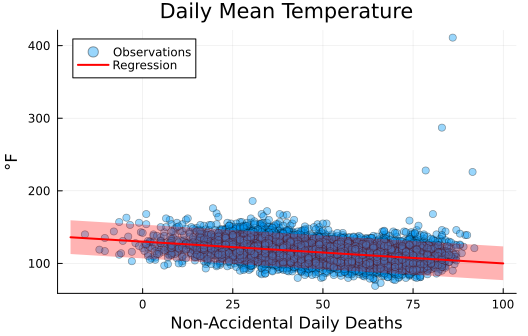
\includegraphics[keepaspectratio]{hw02_files/mediabag/hw02_files/figure-pdf/fig-chicago-tmpd-output-1.pdf}}

}

\caption{\label{fig-chicago-tmpd}Fitted relationship between mean
temperature and non-accidental deaths in Chicago. The shaded region is
the 90\% prediction interval from the linear regression model.}

\end{figure}%

The general trend in Figure~\ref{fig-chicago-tmpd} looks reasonable. We
can calculate the surprise index by finding the fraction of observations
which are outside of the 90\% prediction interval.

\phantomsection\label{annotated-cell-8}%
\begin{Shaded}
\begin{Highlighting}[]
\NormalTok{resids }\OperatorTok{=}\NormalTok{ chicago\_dat.death }\OperatorTok{{-}}\NormalTok{ (b0 }\OperatorTok{.+}\NormalTok{ b1 }\OperatorTok{*}\NormalTok{ chicago\_dat.tmpd)}
\NormalTok{si }\OperatorTok{=} \FunctionTok{sum}\NormalTok{((resids }\OperatorTok{.\textless{}}\NormalTok{ err\_quantile[}\FloatTok{1}\NormalTok{]) }\OperatorTok{+}\NormalTok{ (resids }\OperatorTok{.\textgreater{}}\NormalTok{ err\_quantile[}\FloatTok{2}\NormalTok{])) }\OperatorTok{/} \FunctionTok{nrow}\NormalTok{(chicago\_dat) }\hspace*{\fill}\NormalTok{\circled{1}}
\FunctionTok{round}\NormalTok{(si; digits}\OperatorTok{=}\FloatTok{2}\NormalTok{)}
\end{Highlighting}
\end{Shaded}

\begin{description}
\tightlist
\item[\circled{1}]
The \texttt{sum} term here will add together two vectors, one of which
is 1 when the residuals are below the lower bound of the interval, and
the second which is 1 when they're above the upper bound.
\end{description}

\begin{verbatim}
0.07
\end{verbatim}

The surprise index is about 8\%, which is not ideal, but also isn't so
far from the expected 10\% to be indicative of a major problem. Let's
look at the distribution of residuals and a Q-Q plot to see if the
residuals appear normal.

\begin{Shaded}
\begin{Highlighting}[]
\NormalTok{resid\_hist }\OperatorTok{=} \FunctionTok{histogram}\NormalTok{(resids, xlabel}\OperatorTok{=}\StringTok{"Residuals"}\NormalTok{, ylabel}\OperatorTok{=}\StringTok{"Count"}\NormalTok{, legend}\OperatorTok{=}\ConstantTok{false}\NormalTok{)}
\NormalTok{resid\_qq }\OperatorTok{=} \FunctionTok{qqplot}\NormalTok{(resids, }\FunctionTok{Normal}\NormalTok{(), xlabel}\OperatorTok{=}\StringTok{"Theoretical Quantiles"}\NormalTok{, ylabel}\OperatorTok{=}\StringTok{"Empirical Quantiles"}\NormalTok{)}
\NormalTok{p }\OperatorTok{=} \FunctionTok{plot}\NormalTok{(resid\_hist, resid\_qq, layout}\OperatorTok{=}\NormalTok{(}\FloatTok{2}\NormalTok{, }\FloatTok{1}\NormalTok{))}
\end{Highlighting}
\end{Shaded}

\begin{figure}[H]

\centering{

\pandocbounded{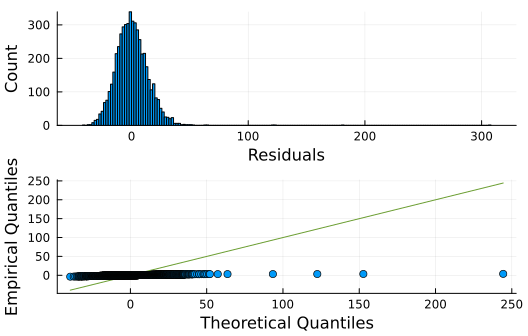
\includegraphics[keepaspectratio]{hw02_files/mediabag/hw02_files/figure-pdf/fig-chicago-diagnostic-output-1.pdf}}

}

\caption{\label{fig-chicago-diagnostic}Diagnostics to check Gaussian
assumptions for the residuals.}

\end{figure}%

Figure~\ref{fig-chicago-diagnostic} suggests that while the bulk of the
residuals appear to follow a Gaussian distribution, there is a long
upper tail which throws off the Q-Q plot. From
Figure~\ref{fig-chicago-tmpd}, these large outliers occur at very high
temperatures; the simple regression model cannot account for this change
in trend, which could be due to extreme heat exposure or some other
factor which is correlated with high temperatures. We might trust this
model for temperatures below 80\(^\circ\) F, or we would want to rethink
the model completely with a better representation of factors which
contribute to deaths.

\subsubsection{Problem 2 (6 points)}\label{problem-2-6-points}

\paragraph{Problem 2.1}\label{problem-2.1}

Denoting the occurrence of freezing in year \(i\) as \(y_i\), the
probability of this occurring as \(p_i\), and the DJF temperature as
\(T\), the logistic regression model can be formulated as:

\[\begin{aligned}
y_i &\sim \text{Binomial}(p_i) \\
\text{logit}(p_i) &= \beta_0 + \beta_1 T.
\end{aligned}\]

Let's load the data and calculate the winter temperatures. I decided to
write a function which would calculate the DJF mean for a given base
year, which would allow me to loop over all of the years and apply the
function; there are many other possible approaches one could take.

\phantomsection\label{annotated-cell-10}%
\begin{Shaded}
\begin{Highlighting}[]
\NormalTok{temp\_dat }\OperatorTok{=}\NormalTok{ CSV.}\FunctionTok{read}\NormalTok{(}\StringTok{"data/HadCRUT5.1Analysis\_gl.txt"}\NormalTok{, delim}\OperatorTok{=}\StringTok{" "}\NormalTok{, ignorerepeated}\OperatorTok{=}\ConstantTok{true}\NormalTok{, header}\OperatorTok{=}\ConstantTok{false}\NormalTok{, silencewarnings}\OperatorTok{=}\ConstantTok{true}\NormalTok{, DataFrame) }\hspace*{\fill}\NormalTok{\circled{1}}
\NormalTok{temp\_dat }\OperatorTok{=}\NormalTok{ temp\_dat[}\FloatTok{1}\OperatorTok{:}\FloatTok{2}\OperatorTok{:}\FunctionTok{nrow}\NormalTok{(temp\_dat), }\OperatorTok{:}\NormalTok{] }\CommentTok{\# only keep even rows}

\KeywordTok{function} \FunctionTok{djf\_mean}\NormalTok{(temps, year)}
\NormalTok{    idx }\OperatorTok{=} \FunctionTok{findfirst}\NormalTok{(temps[}\OperatorTok{:}\NormalTok{, }\FloatTok{1}\NormalTok{] }\OperatorTok{.==}\NormalTok{ year) }\hspace*{\fill}\NormalTok{\circled{2}}
    \ControlFlowTok{return} \FunctionTok{mean}\NormalTok{([temps[idx }\OperatorTok{{-}} \FloatTok{1}\NormalTok{, }\FloatTok{13}\NormalTok{], temps[idx, }\FloatTok{2}\NormalTok{], temps[idx, }\FloatTok{3}\NormalTok{]]) }\hspace*{\fill}\NormalTok{\circled{3}}
\KeywordTok{end}

\NormalTok{djf\_means }\OperatorTok{=}\NormalTok{ [}\FunctionTok{djf\_mean}\NormalTok{(temp\_dat, yr) for yr }\KeywordTok{in} \FloatTok{1851}\OperatorTok{:}\FloatTok{2025}\NormalTok{] }\hspace*{\fill}\NormalTok{\circled{4}}
\end{Highlighting}
\end{Shaded}

\begin{description}
\tightlist
\item[\circled{1}]
We need \texttt{silencewarnings=true} because \texttt{CSV.read} will
complain about the even rows not having the same number of columns.
\item[\circled{2}]
\texttt{findfirst} (or the equivalent) is the fastest solution since it
will terminate after finding any matches, but if you used a different
approach which involved searching over the entire \texttt{DataFrame}, it
wouldn't matter too much in this case since the data is small.
\item[\circled{3}]
\texttt{temps{[}idx\ -\ 1,\ 13{]}} is the previous December since the
first column is the year, and similarly for that year's January and
February.
\item[\circled{4}]
This is a straightforward use of a comprehension to apply a function in
a loop. Comprehensions are quite memory efficient. There are other
strategies, such as mapping the function, that one could use.
\end{description}

\begin{verbatim}
175-element Vector{Float64}:
 -0.35166666666666674
 -0.3633333333333333
 -0.17966666666666667
 -0.37366666666666665
 -0.31233333333333335
 -0.2793333333333333
 -0.453
 -0.371
 -0.4036666666666667
 -0.393
  ⋮
  0.9269999999999999
  0.7629999999999999
  0.8213333333333334
  1.0646666666666667
  0.6546666666666666
  0.7643333333333334
  0.8046666666666668
  1.2286666666666666
  1.167
\end{verbatim}

Now we want to create a vector of \texttt{1}s and \texttt{0}s for the
freezing occurrences and non-occurrences (as a reminder, 1796 and 1816
are outside of the temperature data, so we will not include those).
We'll put all of the data together in a \texttt{DataFrame} to make it
easy to assign the relevant \texttt{1}s.

\begin{Shaded}
\begin{Highlighting}[]
\NormalTok{freezes }\OperatorTok{=}\NormalTok{ [}\FloatTok{1856}\NormalTok{, }\FloatTok{1875}\NormalTok{, }\FloatTok{1884}\NormalTok{, }\FloatTok{1904}\NormalTok{, }\FloatTok{1912}\NormalTok{, }\FloatTok{1934}\NormalTok{, }\FloatTok{1961}\NormalTok{, }\FloatTok{1979}\NormalTok{, }\FloatTok{2015}\NormalTok{]}
\NormalTok{dat }\OperatorTok{=} \FunctionTok{DataFrame}\NormalTok{(year}\OperatorTok{=}\FloatTok{1851}\OperatorTok{:}\FloatTok{2025}\NormalTok{, temp}\OperatorTok{=}\NormalTok{djf\_means, freeze}\OperatorTok{=}\FunctionTok{zeros}\NormalTok{(}\FunctionTok{length}\NormalTok{(djf\_means)))}
\ControlFlowTok{for}\NormalTok{ yr }\KeywordTok{in}\NormalTok{ freezes}
\NormalTok{    idx }\OperatorTok{=} \FunctionTok{findfirst}\NormalTok{(dat.year }\OperatorTok{.==}\NormalTok{ yr)}
\NormalTok{    dat[idx, }\OperatorTok{:}\NormalTok{freeze] }\OperatorTok{=} \FloatTok{1}
\ControlFlowTok{end}
\end{Highlighting}
\end{Shaded}

Now let's maximize the likelihood of the model. We need to be able to
compute the inverse logit of the linear part of the model, which is
given by \[\text{logit}^{-1}(x) = \frac{\exp(x)}{\exp(x) + 1}.\]

\begin{Shaded}
\begin{Highlighting}[]
\FunctionTok{logit}\NormalTok{(p) }\OperatorTok{=} \FunctionTok{log}\NormalTok{(p }\OperatorTok{/}\NormalTok{ (}\FloatTok{1} \OperatorTok{{-}}\NormalTok{ p))}
\FunctionTok{invlogit}\NormalTok{(x) }\OperatorTok{=} \FunctionTok{exp}\NormalTok{(x) }\OperatorTok{/}\NormalTok{ (}\FunctionTok{exp}\NormalTok{(x) }\OperatorTok{+} \FloatTok{1}\NormalTok{)}
\KeywordTok{function} \FunctionTok{freeze\_loglik}\NormalTok{(params, dat)}
\NormalTok{    b0, b1 }\OperatorTok{=}\NormalTok{ params}
\NormalTok{    p }\OperatorTok{=} \FunctionTok{invlogit}\NormalTok{.(b0 }\OperatorTok{.+}\NormalTok{ b1 }\OperatorTok{*}\NormalTok{ dat.temp)}
\NormalTok{    ll }\OperatorTok{=} \FunctionTok{sum}\NormalTok{(}\FunctionTok{logpdf}\NormalTok{.(}\FunctionTok{Bernoulli}\NormalTok{.(p), dat.freeze))}
    \ControlFlowTok{return}\NormalTok{ ll}
\KeywordTok{end}

\NormalTok{lb }\OperatorTok{=}\NormalTok{ [}\OperatorTok{{-}}\FloatTok{20.0}\NormalTok{, }\OperatorTok{{-}}\FloatTok{20.0}\NormalTok{]}
\NormalTok{ub }\OperatorTok{=}\NormalTok{ [}\FloatTok{20.0}\NormalTok{, }\FloatTok{20.0}\NormalTok{]}
\NormalTok{p0 }\OperatorTok{=}\NormalTok{ [}\FloatTok{0.25}\NormalTok{, }\FloatTok{0.25}\NormalTok{]}
\NormalTok{optim\_out }\OperatorTok{=}\NormalTok{ Optim.}\FunctionTok{optimize}\NormalTok{(v }\OperatorTok{{-}\textgreater{}} \FunctionTok{{-}freeze\_loglik}\NormalTok{(v, dat), lb, ub, p0)}
\NormalTok{v\_mle }\OperatorTok{=} \FunctionTok{round}\NormalTok{.(optim\_out.minimizer; digits}\OperatorTok{=}\FloatTok{1}\NormalTok{)}
\end{Highlighting}
\end{Shaded}

\begin{verbatim}
2-element Vector{Float64}:
 -3.0
 -0.7
\end{verbatim}

We can interpret these coefficients as follows:

\begin{itemize}
\tightlist
\item
  \(\hat{\beta}_0 = -3\) gives us the probability of freezing when the
  temperature anomaly is the same as the reference period mean, namely
  \(\text{logit}^{-1}(-3) = 4.7\%\).
\item
  \(\hat{\beta}_1 = -0.7\) gives the reduction in freezing log-odds
  associated with a temperature anomaly increase of \(1^\circ\) C. It's
  not entirely clear what this means, but one important feature is that
  this is negative, so that increased temperatures decrease the
  probability of freezing, which is what we would expect.
\end{itemize}

\paragraph{Problem 2.2}\label{problem-2.2}

Let's plot how the probability of freezing changes with respect to
temperature and time.

\begin{Shaded}
\begin{Highlighting}[]
\NormalTok{temp\_pred }\OperatorTok{=} \OperatorTok{{-}}\FloatTok{1}\OperatorTok{:}\FloatTok{0.1}\OperatorTok{:}\FloatTok{2}
\NormalTok{p1 }\OperatorTok{=} \FunctionTok{plot}\NormalTok{(}\OperatorTok{{-}}\FloatTok{1}\OperatorTok{:}\FloatTok{0.1}\OperatorTok{:}\FloatTok{2}\NormalTok{, }\FunctionTok{invlogit}\NormalTok{.(v\_mle[}\FloatTok{1}\NormalTok{] }\OperatorTok{.+}\NormalTok{ v\_mle[}\FloatTok{2}\NormalTok{] }\OperatorTok{*}\NormalTok{ temp\_pred), xlabel}\OperatorTok{=}\StringTok{"DJF Temperature Anomaly (°C)"}\NormalTok{, ylabel}\OperatorTok{=}\StringTok{"Probability Cayuga Lake Freezes"}\NormalTok{, legend}\OperatorTok{=}\ConstantTok{false}\NormalTok{)}
\NormalTok{p2 }\OperatorTok{=} \FunctionTok{plot}\NormalTok{(dat.year, }\FunctionTok{invlogit}\NormalTok{.(v\_mle[}\FloatTok{1}\NormalTok{] }\OperatorTok{.+}\NormalTok{ v\_mle[}\FloatTok{2}\NormalTok{] }\OperatorTok{*}\NormalTok{ dat.temp), xlabel}\OperatorTok{=}\StringTok{"Year"}\NormalTok{, ylabel}\OperatorTok{=}\StringTok{"Probability Cayuga Lake Freezes"}\NormalTok{)}
\FunctionTok{plot}\NormalTok{(p1, p2, layout}\OperatorTok{=}\NormalTok{(}\FloatTok{1}\NormalTok{, }\FloatTok{2}\NormalTok{), legend}\OperatorTok{=}\ConstantTok{false}\NormalTok{)}
\end{Highlighting}
\end{Shaded}

\begin{figure}[H]

\centering{

\pandocbounded{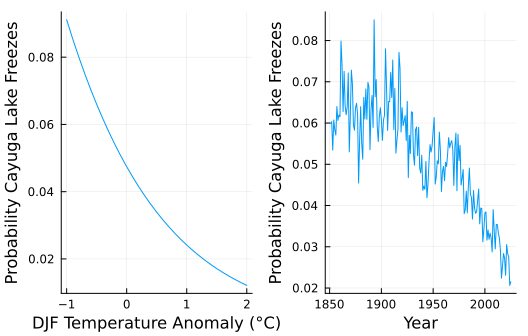
\includegraphics[keepaspectratio]{hw02_files/mediabag/hw02_files/figure-pdf/fig-freezing-temps-output-1.pdf}}

}

\caption{\label{fig-freezing-temps}Modeled probability of Cayuga Lake
freezing versus the DJF temperature anomaly and over time.}

\end{figure}%

We can see from Figure~\ref{fig-freezing-temps} that the probability has
declined precipitously over time as the temperature anomaly has
increased, from around a 6-8\% probability between 1851 and 1925 down to
around 2\% today.

How can we determine if this model is reasonable? Since the
probabilities of occurrence are so low, we can't try to look at a raw
mis-classification rate. However, we can try to assess how well
calibrated the model is, \emph{e.g.}, does it generally predict the
right number of freezes. We have observed 9 years in which Cayuga Lake
has frozen (that align with our temperature data); let's see if the
expected number of freezes is similar to this by adding up the modeled
probabilities.

\begin{Shaded}
\begin{Highlighting}[]
\NormalTok{p\_fit }\OperatorTok{=} \FunctionTok{invlogit}\NormalTok{.(v\_mle[}\FloatTok{1}\NormalTok{] }\OperatorTok{.+}\NormalTok{ v\_mle[}\FloatTok{2}\NormalTok{] }\OperatorTok{*}\NormalTok{ dat.temp)}
\FunctionTok{sum}\NormalTok{(p\_fit)}
\end{Highlighting}
\end{Shaded}

\begin{verbatim}
9.116926466107916
\end{verbatim}

This is almost exactly right, though it is a bit generous to the model
because it's an in-sample estimate. We can also look at how well the
model captures probabilities of freezing at different ranges of
predicted probabilities. Let's look at what happens between
probabilities over 5\% and under 5\%.

\begin{Shaded}
\begin{Highlighting}[]
\FunctionTok{sum}\NormalTok{(p\_fit[p\_fit }\OperatorTok{.\textgreater{}} \FloatTok{0.05}\NormalTok{])}
\end{Highlighting}
\end{Shaded}

\begin{verbatim}
6.511824596882027
\end{verbatim}

\begin{Shaded}
\begin{Highlighting}[]
\FunctionTok{sum}\NormalTok{(dat.freeze[p\_fit }\OperatorTok{.\textgreater{}} \FloatTok{0.05}\NormalTok{])}
\end{Highlighting}
\end{Shaded}

\begin{verbatim}
6.0
\end{verbatim}

That's off by a little, but not much.

Similarly, for probabilities below 5\%:

\begin{Shaded}
\begin{Highlighting}[]
\FunctionTok{sum}\NormalTok{(p\_fit[p\_fit }\OperatorTok{.\textless{}} \FloatTok{0.05}\NormalTok{])}
\end{Highlighting}
\end{Shaded}

\begin{verbatim}
2.605101869225891
\end{verbatim}

\begin{Shaded}
\begin{Highlighting}[]
\FunctionTok{sum}\NormalTok{(dat.freeze[p\_fit }\OperatorTok{.\textless{}} \FloatTok{0.05}\NormalTok{])}
\end{Highlighting}
\end{Shaded}

\begin{verbatim}
3.0
\end{verbatim}

Try out other ranges to see where the model performs well and where it
doesn't: if you see ranges where the model substantially over or under
predicts, that's a signal of mis-specification.

Beyond this, diagnosing logistic regression \emph{post facto} can be
difficult because it doesn't make distributional assumptions; you need
to convince yourself that the log-odds ought to have a linear
relationship with the predictor(s), which can be difficult.

\paragraph{Problem 2.3}\label{problem-2.3}

To find the temperature required for less than a 1\% probability of
Cayuga Lake freezing, we need to find \(\text{logit}(0.01)\) and solve
for the temperature based on the logistic regression.

\begin{Shaded}
\begin{Highlighting}[]
\NormalTok{freeze\_thresh\_prob }\OperatorTok{=} \FunctionTok{logit}\NormalTok{(}\FloatTok{0.01}\NormalTok{)}
\NormalTok{freeze\_thresh\_temp }\OperatorTok{=}\NormalTok{ (freeze\_thresh\_prob }\OperatorTok{{-}}\NormalTok{ v\_mle[}\FloatTok{1}\NormalTok{]) }\OperatorTok{/}\NormalTok{ v\_mle[}\FloatTok{2}\NormalTok{]}
\end{Highlighting}
\end{Shaded}

\begin{verbatim}
2.278742643049414
\end{verbatim}

So if the winter temperature anomaly rises above 2.2\(^\circ\) C, we
would expect the probability of Cayuga Lake freezing to drop below 1\%.

\subsubsection{Problem 3 (6 points)}\label{problem-3-6-points}

The file \texttt{data/salamanders.csv} contains counts of salamanders
from 47 different plots of the same area in California, as well as the
percentage of ground cover and age of the forest in the plot. You would
like to see if you can use these data to predict the salamander counts
with a Poisson regression.

\paragraph{Problem 3.1}\label{problem-3.1}

Loading the data (note the delimiter is now a semi-colon):

\begin{Shaded}
\begin{Highlighting}[]
\NormalTok{dat }\OperatorTok{=}\NormalTok{ CSV.}\FunctionTok{read}\NormalTok{(}\FunctionTok{joinpath}\NormalTok{(}\StringTok{"data"}\NormalTok{, }\StringTok{"salamanders.csv"}\NormalTok{), DataFrame, delim}\OperatorTok{=}\StringTok{";"}\NormalTok{)}
\end{Highlighting}
\end{Shaded}

\begin{tabular}{r|cccc}
    & SITE & SALAMAN & PCTCOVER & FORESTAGE\\
    \hline
    & Int64 & Int64 & Int64 & Int64\\
    \hline
    1 & 1 & 13 & 85 & 316 \\
    2 & 2 & 11 & 86 & 88 \\
    3 & 3 & 11 & 90 & 548 \\
    4 & 4 & 9 & 88 & 64 \\
    5 & 5 & 8 & 89 & 43 \\
    6 & 6 & 7 & 83 & 368 \\
    7 & 7 & 6 & 83 & 200 \\
    8 & 8 & 6 & 91 & 71 \\
    9 & 9 & 5 & 88 & 42 \\
    10 & 10 & 5 & 90 & 551 \\
    11 & 11 & 4 & 87 & 675 \\
    12 & 12 & 3 & 83 & 217 \\
    13 & 13 & 3 & 87 & 212 \\
    14 & 14 & 3 & 89 & 398 \\
    15 & 15 & 3 & 92 & 357 \\
    16 & 16 & 3 & 93 & 478 \\
    17 & 17 & 2 & 2 & 5 \\
    18 & 18 & 2 & 87 & 30 \\
    19 & 19 & 2 & 93 & 551 \\
    20 & 20 & 1 & 7 & 3 \\
    21 & 21 & 1 & 16 & 15 \\
    22 & 22 & 1 & 19 & 31 \\
    23 & 23 & 1 & 29 & 10 \\
    24 & 24 & 1 & 34 & 49 \\
    $\dots$ & $\dots$ & $\dots$ & $\dots$ & $\dots$ \\
\end{tabular}

The first model, using \texttt{PCTCOVER} as a predictor, can be
specified as the following (using the standard log link function for
Poisson regression):

\[
\begin{aligned}
S &\sim \text{Poisson}(\lambda) \\
\log(\lambda) &= a PC + b
\end{aligned}
\]

As noted in the problem, we will need to standardize the
\texttt{PCTCOVER} variable, as its range is much larger than the
salamander counts.

\phantomsection\label{annotated-cell-21}%
\begin{Shaded}
\begin{Highlighting}[]
\KeywordTok{function} \FunctionTok{salamander\_pcover}\NormalTok{(p, counts, pctcover) }
\NormalTok{    a, b }\OperatorTok{=}\NormalTok{ p}
\NormalTok{    λ }\OperatorTok{=} \FunctionTok{exp}\NormalTok{.(a }\OperatorTok{*}\NormalTok{ pctcover }\OperatorTok{.+}\NormalTok{ b)}
\NormalTok{    ll }\OperatorTok{=} \FunctionTok{sum}\NormalTok{(}\FunctionTok{logpdf}\NormalTok{.(}\FunctionTok{Poisson}\NormalTok{.(λ), counts))}
    \ControlFlowTok{return}\NormalTok{ ll}
\KeywordTok{end}

\NormalTok{lb }\OperatorTok{=}\NormalTok{ [}\OperatorTok{{-}}\FloatTok{10.0}\NormalTok{, }\OperatorTok{{-}}\FloatTok{50.0}\NormalTok{]}
\NormalTok{ub }\OperatorTok{=}\NormalTok{ [}\FloatTok{10.0}\NormalTok{, }\FloatTok{50.0}\NormalTok{]}
\NormalTok{p0 }\OperatorTok{=}\NormalTok{ [}\FloatTok{0.0}\NormalTok{, }\FloatTok{0.0}\NormalTok{]}

\CommentTok{\# function to make this more convenient}
\FunctionTok{stdz}\NormalTok{(x) }\OperatorTok{=}\NormalTok{ (x }\OperatorTok{.{-}} \FunctionTok{mean}\NormalTok{(x)) }\OperatorTok{/} \FunctionTok{std}\NormalTok{(x) }\hspace*{\fill}\NormalTok{\circled{1}}

\NormalTok{result }\OperatorTok{=} \FunctionTok{optimize}\NormalTok{(p }\OperatorTok{{-}\textgreater{}} \FunctionTok{{-}salamander\_pcover}\NormalTok{(p, dat.SALAMAN, }\FunctionTok{stdz}\NormalTok{(dat.PCTCOVER)), lb, ub, p0)}
\NormalTok{pcover\_mle }\OperatorTok{=} \FunctionTok{round}\NormalTok{.(result.minimizer; digits}\OperatorTok{=}\FloatTok{1}\NormalTok{)}
\end{Highlighting}
\end{Shaded}

\begin{verbatim}
2-element Vector{Float64}:
 1.2
 0.4
\end{verbatim}

\paragraph{Problem 3.2}\label{problem-3.2}

To translate these estimates to expected values and uncertainty
intervals, we now simulate observations of salamanders based on this
model.

\phantomsection\label{annotated-cell-22}%
\begin{Shaded}
\begin{Highlighting}[]
\KeywordTok{function} \FunctionTok{sim\_salamanders\_pcover}\NormalTok{(params, pctcover, n)}
\NormalTok{    a, b }\OperatorTok{=}\NormalTok{ params}
\NormalTok{    λ }\OperatorTok{=} \FunctionTok{exp}\NormalTok{.(a }\OperatorTok{*}\NormalTok{ pctcover }\OperatorTok{.+}\NormalTok{ b)}
\NormalTok{    sal\_pred }\OperatorTok{=} \FunctionTok{zeros}\NormalTok{(n, }\FunctionTok{length}\NormalTok{(pctcover))}
    \ControlFlowTok{for}\NormalTok{ i }\OperatorTok{=} \FloatTok{1}\OperatorTok{:}\FunctionTok{length}\NormalTok{(pctcover)}
\NormalTok{        sal\_pred[}\OperatorTok{:}\NormalTok{, i] }\OperatorTok{=} \FunctionTok{rand}\NormalTok{(}\FunctionTok{Poisson}\NormalTok{(λ[i]), n)}
    \ControlFlowTok{end}
    \ControlFlowTok{return}\NormalTok{ sal\_pred}
\KeywordTok{end}

\NormalTok{sim\_pcover }\OperatorTok{=} \FunctionTok{sim\_salamanders\_pcover}\NormalTok{(pcover\_mle, }\OperatorTok{{-}}\FloatTok{2}\OperatorTok{:}\FloatTok{0.01}\OperatorTok{:}\FloatTok{2}\NormalTok{, }\FloatTok{10\_000}\NormalTok{) }\hspace*{\fill}\NormalTok{\circled{1}}

\NormalTok{pcover\_q }\OperatorTok{=} \FunctionTok{mapslices}\NormalTok{(col }\OperatorTok{{-}\textgreater{}} \FunctionTok{quantile}\NormalTok{(col, [}\FloatTok{0.05}\NormalTok{, }\FloatTok{0.5}\NormalTok{, }\FloatTok{0.95}\NormalTok{]), sim\_pcover; dims}\OperatorTok{=}\FloatTok{1}\NormalTok{) }
\FunctionTok{plot}\NormalTok{(}\OperatorTok{{-}}\FloatTok{2}\OperatorTok{:}\FloatTok{0.01}\OperatorTok{:}\FloatTok{2}\NormalTok{, pcover\_q[}\FloatTok{2}\NormalTok{, }\OperatorTok{:}\NormalTok{], linewidth}\OperatorTok{=}\FloatTok{3}\NormalTok{, ribbon}\OperatorTok{=}\NormalTok{(pcover\_q[}\FloatTok{2}\NormalTok{, }\OperatorTok{:}\NormalTok{] }\OperatorTok{{-}}\NormalTok{ pcover\_q[}\FloatTok{1}\NormalTok{, }\OperatorTok{:}\NormalTok{], pcover\_q[}\FloatTok{3}\NormalTok{, }\OperatorTok{:}\NormalTok{] }\OperatorTok{{-}}\NormalTok{ pcover\_q[}\FloatTok{2}\NormalTok{, }\OperatorTok{:}\NormalTok{]), fillalpha}\OperatorTok{=}\FloatTok{0.5}\NormalTok{, xlabel}\OperatorTok{=}\StringTok{"Standardized Percent Ground Cover"}\NormalTok{, ylabel}\OperatorTok{=}\StringTok{"Salamander Count"}\NormalTok{, label}\OperatorTok{=}\StringTok{"Simulations"}\NormalTok{) }
\FunctionTok{scatter!}\NormalTok{(}\FunctionTok{stdz}\NormalTok{(dat.PCTCOVER), dat.SALAMAN, label}\OperatorTok{=}\StringTok{"Observations"}\NormalTok{)}
\end{Highlighting}
\end{Shaded}

\begin{description}
\tightlist
\item[\circled{1}]
Note that our predictors are along the \textbf{standardized} predictor
range, not the \emph{raw} \texttt{PCTCOVER} range, since we standardized
the inputs when we fit the regression.
\end{description}

\begin{figure}[H]

\centering{

\pandocbounded{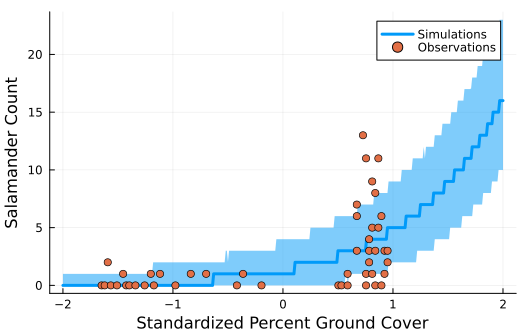
\includegraphics[keepaspectratio]{hw02_files/mediabag/hw02_files/figure-pdf/fig-salamander-sim-output-1.pdf}}

}

\caption{\label{fig-salamander-sim}Predictive interval of salamander
counts using the percent cover model.}

\end{figure}%

The model seems to do ok for lower levels of percent cover, but does not
account for the level of dispersion at higher levels; this might suggest
that a Poisson model is not ideal, but we could try a negative binomial
regression instead.

\paragraph{Problem 3.3}\label{problem-3.3}

Let's see if we can improve the model using the \texttt{FORESTAGE}
predictor. We'll try to add this in as a linear predictor.

\begin{Shaded}
\begin{Highlighting}[]
\KeywordTok{function} \FunctionTok{salamander\_fage}\NormalTok{(p, counts, pctcover, forestage) }
\NormalTok{    a1, a2, b }\OperatorTok{=}\NormalTok{ p}
\NormalTok{    λ }\OperatorTok{=} \FunctionTok{exp}\NormalTok{.(a1 }\OperatorTok{*}\NormalTok{ pctcover }\OperatorTok{+}\NormalTok{ a2 }\OperatorTok{*}\NormalTok{ forestage }\OperatorTok{.+}\NormalTok{ b)}
\NormalTok{    ll }\OperatorTok{=} \FunctionTok{sum}\NormalTok{(}\FunctionTok{logpdf}\NormalTok{.(}\FunctionTok{Poisson}\NormalTok{.(λ), counts))}
    \ControlFlowTok{return}\NormalTok{ ll}
\KeywordTok{end}

\NormalTok{lb }\OperatorTok{=}\NormalTok{ [}\OperatorTok{{-}}\FloatTok{10.0}\NormalTok{, }\OperatorTok{{-}}\FloatTok{10.0}\NormalTok{, }\OperatorTok{{-}}\FloatTok{50.0}\NormalTok{]}
\NormalTok{ub }\OperatorTok{=}\NormalTok{ [}\FloatTok{10.0}\NormalTok{, }\FloatTok{10.0}\NormalTok{, }\FloatTok{50.0}\NormalTok{]}
\NormalTok{p0 }\OperatorTok{=}\NormalTok{ [}\FloatTok{0.0}\NormalTok{, }\FloatTok{0.0}\NormalTok{, }\FloatTok{0.0}\NormalTok{]}

\NormalTok{result }\OperatorTok{=} \FunctionTok{optimize}\NormalTok{(p }\OperatorTok{{-}\textgreater{}} \FunctionTok{{-}salamander\_fage}\NormalTok{(p, dat.SALAMAN, }\FunctionTok{stdz}\NormalTok{(dat.PCTCOVER), }\FunctionTok{stdz}\NormalTok{(dat.FORESTAGE)), lb, ub, p0)}
\NormalTok{fage\_mle }\OperatorTok{=} \FunctionTok{round}\NormalTok{.(result.minimizer; digits}\OperatorTok{=}\FloatTok{1}\NormalTok{)}
\end{Highlighting}
\end{Shaded}

\begin{verbatim}
3-element Vector{Float64}:
  1.2
 -0.0
  0.4
\end{verbatim}

We can see that the \texttt{FORESTAGE} predictor variable is effectively
zero, which means it does not add much to the prediction. Why is this?
The correlation between \texttt{PCTCOVER} and \texttt{FORESTAGE} is
quite high: 0.63, which means most of the information in
\texttt{FORESTAGE} has already been included in the \texttt{PCTCOVER}
model. It makes sense that \texttt{PCTCOVER} is valuable: salamanders
are likely to seek areas with high levels of ground cover, while the age
of the forest is only meaningful to the extent that older forests may
have more ground cover (hence the high correlation).

\subsubsection{Problem 4 (7 points)}\label{problem-4-7-points}

\paragraph{Problem 4.1}\label{problem-4.1}

Loading the data (once again, the file is delimited by semi-colons):

\begin{Shaded}
\begin{Highlighting}[]
\NormalTok{dat }\OperatorTok{=}\NormalTok{ CSV.}\FunctionTok{read}\NormalTok{(}\FunctionTok{joinpath}\NormalTok{(}\StringTok{"data"}\NormalTok{, }\StringTok{"Hurricanes.csv"}\NormalTok{), DataFrame, delim}\OperatorTok{=}\StringTok{";"}\NormalTok{)}
\end{Highlighting}
\end{Shaded}

\begin{tabular}{r|cccccccc}
    & name & year & deaths & category & min\_pressure & damage\_norm & female & femininity\\
    \hline
    & String15 & Int64 & Int64 & Int64 & Int64 & Int64 & Int64 & Float64\\
    \hline
    1 & Easy & 1950 & 2 & 3 & 960 & 1590 & 1 & 6.77778 \\
    2 & King & 1950 & 4 & 3 & 955 & 5350 & 0 & 1.38889 \\
    3 & Able & 1952 & 3 & 1 & 985 & 150 & 0 & 3.83333 \\
    4 & Barbara & 1953 & 1 & 1 & 987 & 58 & 1 & 9.83333 \\
    5 & Florence & 1953 & 0 & 1 & 985 & 15 & 1 & 8.33333 \\
    6 & Carol & 1954 & 60 & 3 & 960 & 19321 & 1 & 8.11111 \\
    7 & Edna & 1954 & 20 & 3 & 954 & 3230 & 1 & 8.55556 \\
    8 & Hazel & 1954 & 20 & 4 & 938 & 24260 & 1 & 9.44444 \\
    9 & Connie & 1955 & 0 & 3 & 962 & 2030 & 1 & 8.5 \\
    10 & Diane & 1955 & 200 & 1 & 987 & 14730 & 1 & 9.88889 \\
    11 & Ione & 1955 & 7 & 3 & 960 & 6200 & 0 & 5.94444 \\
    12 & Flossy & 1956 & 15 & 2 & 975 & 1540 & 1 & 7.0 \\
    13 & Helene & 1958 & 1 & 3 & 946 & 540 & 1 & 9.88889 \\
    14 & Debra & 1959 & 0 & 1 & 984 & 430 & 1 & 9.88889 \\
    15 & Gracie & 1959 & 22 & 3 & 950 & 510 & 1 & 9.77778 \\
    16 & Donna & 1960 & 50 & 4 & 930 & 53270 & 1 & 9.27778 \\
    17 & Ethel & 1960 & 0 & 1 & 981 & 35 & 1 & 8.72222 \\
    18 & Carla & 1961 & 46 & 4 & 931 & 15850 & 1 & 9.5 \\
    19 & Cindy & 1963 & 3 & 1 & 996 & 300 & 1 & 9.94444 \\
    20 & Cleo & 1964 & 3 & 2 & 968 & 6450 & 1 & 7.94444 \\
    21 & Dora & 1964 & 5 & 2 & 966 & 16260 & 1 & 9.33333 \\
    22 & Hilda & 1964 & 37 & 3 & 950 & 2770 & 1 & 8.83333 \\
    23 & Isbell & 1964 & 3 & 2 & 974 & 800 & 1 & 9.44444 \\
    24 & Betsy & 1965 & 75 & 3 & 948 & 20000 & 1 & 8.33333 \\
    $\dots$ & $\dots$ & $\dots$ & $\dots$ & $\dots$ & $\dots$ & $\dots$ & $\dots$ & $\dots$ \\
\end{tabular}

Our interpretation of the hypothesis results in the following model
specification:

\[
\begin{aligned}
D &\sim \text{Poisson}(\lambda) \\
\log(\lambda) &= a_1 FN + a_2 MP + b
\end{aligned}
\]

We need to standardized the pressure predictor.

\phantomsection\label{annotated-cell-25}%
\begin{Shaded}
\begin{Highlighting}[]
\KeywordTok{function} \FunctionTok{hurricane\_pressure}\NormalTok{(p, counts, fem, pressure) }
\NormalTok{    a1, a2, b }\OperatorTok{=}\NormalTok{ p}
\NormalTok{    m }\OperatorTok{=} \FunctionTok{exp}\NormalTok{.(a1 }\OperatorTok{*}\NormalTok{ fem }\OperatorTok{+}\NormalTok{ a2 }\OperatorTok{*}\NormalTok{ pressure }\OperatorTok{.+}\NormalTok{ b)}
\NormalTok{    ll }\OperatorTok{=} \FunctionTok{sum}\NormalTok{(}\FunctionTok{logpdf}\NormalTok{.(}\FunctionTok{Poisson}\NormalTok{.(m), counts))}
    \ControlFlowTok{return}\NormalTok{ ll}
\KeywordTok{end}

\NormalTok{lb }\OperatorTok{=}\NormalTok{ [}\OperatorTok{{-}}\FloatTok{10.0}\NormalTok{, }\OperatorTok{{-}}\FloatTok{10.0}\NormalTok{, }\OperatorTok{{-}}\FloatTok{50.0}\NormalTok{]}
\NormalTok{ub }\OperatorTok{=}\NormalTok{ [}\FloatTok{10.0}\NormalTok{, }\FloatTok{10.0}\NormalTok{, }\FloatTok{50.0}\NormalTok{]}
\NormalTok{p0 }\OperatorTok{=}\NormalTok{ [}\FloatTok{5.0}\NormalTok{, }\FloatTok{5.0}\NormalTok{, }\FloatTok{0.0}\NormalTok{]}

\CommentTok{\# function to make this more convenient}
\FunctionTok{stdz}\NormalTok{(x) }\OperatorTok{=}\NormalTok{ (x }\OperatorTok{.{-}} \FunctionTok{mean}\NormalTok{(x)) }\OperatorTok{/} \FunctionTok{std}\NormalTok{(x) }\hspace*{\fill}\NormalTok{\circled{1}}

\NormalTok{result }\OperatorTok{=} \FunctionTok{optimize}\NormalTok{(p }\OperatorTok{{-}\textgreater{}} \FunctionTok{{-}hurricane\_pressure}\NormalTok{(p, dat.deaths, dat.female, }\FunctionTok{stdz}\NormalTok{(dat.min\_pressure)), lb, ub, p0)}
\NormalTok{p\_pressure }\OperatorTok{=}\NormalTok{ result.minimizer}
\end{Highlighting}
\end{Shaded}

\begin{verbatim}
3-element Vector{Float64}:
  0.47211173924356337
 -0.7195324699559839
  2.414667236694508
\end{verbatim}

\paragraph{Problem 4.2}\label{problem-4.2}

\phantomsection\label{annotated-cell-26}%
\begin{Shaded}
\begin{Highlighting}[]
\KeywordTok{function} \FunctionTok{sim\_hurricanes}\NormalTok{(p, fem, damage,  n)}
\NormalTok{    a1, a2, b }\OperatorTok{=}\NormalTok{ p}
\NormalTok{    λ }\OperatorTok{=} \FunctionTok{exp}\NormalTok{.(a1 }\OperatorTok{*}\NormalTok{ fem }\OperatorTok{+}\NormalTok{ a2 }\OperatorTok{*}\NormalTok{ damage }\OperatorTok{.+}\NormalTok{ b)}
\NormalTok{    hur\_pred }\OperatorTok{=} \FunctionTok{zeros}\NormalTok{(n, }\FunctionTok{length}\NormalTok{(fem))}
    \ControlFlowTok{for}\NormalTok{ i }\OperatorTok{=} \FloatTok{1}\OperatorTok{:}\FunctionTok{length}\NormalTok{(fem)}
\NormalTok{        hur\_pred[}\OperatorTok{:}\NormalTok{, i] }\OperatorTok{=} \FunctionTok{rand}\NormalTok{(}\FunctionTok{Poisson}\NormalTok{(λ[i]), n)}
    \ControlFlowTok{end}
    \ControlFlowTok{return}\NormalTok{ hur\_pred}
\KeywordTok{end}

\NormalTok{press\_range }\OperatorTok{=} \OperatorTok{{-}}\FloatTok{3}\OperatorTok{:}\FloatTok{0.01}\OperatorTok{:}\FloatTok{2} \CommentTok{\# these are normalized pressures}
\NormalTok{sim\_m }\OperatorTok{=} \FunctionTok{sim\_hurricanes}\NormalTok{(p\_pressure, }\FunctionTok{repeat}\NormalTok{([}\OperatorTok{{-}}\FloatTok{1}\NormalTok{], }\FunctionTok{length}\NormalTok{(press\_range)), press\_range, }\FloatTok{10\_000}\NormalTok{) }\hspace*{\fill}\NormalTok{\circled{1}}
\NormalTok{sim\_f }\OperatorTok{=} \FunctionTok{sim\_hurricanes}\NormalTok{(p\_pressure, }\FunctionTok{repeat}\NormalTok{([}\FloatTok{1}\NormalTok{], }\FunctionTok{length}\NormalTok{(press\_range)), press\_range, }\FloatTok{10\_000}\NormalTok{) }

\NormalTok{simm\_q }\OperatorTok{=} \FunctionTok{mapslices}\NormalTok{(col }\OperatorTok{{-}\textgreater{}} \FunctionTok{quantile}\NormalTok{(col, [}\FloatTok{0.05}\NormalTok{, }\FloatTok{0.5}\NormalTok{, }\FloatTok{0.95}\NormalTok{]), sim\_m; dims}\OperatorTok{=}\FloatTok{1}\NormalTok{)}
\NormalTok{simf\_q }\OperatorTok{=} \FunctionTok{mapslices}\NormalTok{(col }\OperatorTok{{-}\textgreater{}} \FunctionTok{quantile}\NormalTok{(col, [}\FloatTok{0.05}\NormalTok{, }\FloatTok{0.5}\NormalTok{, }\FloatTok{0.95}\NormalTok{]), sim\_f; dims}\OperatorTok{=}\FloatTok{1}\NormalTok{)}

\NormalTok{std\_pressure }\OperatorTok{=} \FunctionTok{stdz}\NormalTok{(dat.min\_pressure)}
\FunctionTok{plot}\NormalTok{(}\OperatorTok{{-}}\FloatTok{3}\OperatorTok{:}\FloatTok{0.01}\OperatorTok{:}\FloatTok{2}\NormalTok{, simm\_q[}\FloatTok{2}\NormalTok{, }\OperatorTok{:}\NormalTok{], linewidth}\OperatorTok{=}\FloatTok{3}\NormalTok{, ribbon}\OperatorTok{=}\NormalTok{(simm\_q[}\FloatTok{2}\NormalTok{, }\OperatorTok{:}\NormalTok{] }\OperatorTok{{-}}\NormalTok{ simm\_q[}\FloatTok{1}\NormalTok{, }\OperatorTok{:}\NormalTok{], simm\_q[}\FloatTok{3}\NormalTok{, }\OperatorTok{:}\NormalTok{] }\OperatorTok{{-}}\NormalTok{ simm\_q[}\FloatTok{2}\NormalTok{, }\OperatorTok{:}\NormalTok{]), alpha}\OperatorTok{=}\FloatTok{0.5}\NormalTok{, label}\OperatorTok{=}\StringTok{"Masculine Storms (Simulation)"}\NormalTok{, color}\OperatorTok{=:}\NormalTok{blue, xlabel}\OperatorTok{=}\StringTok{"Standardized Minimum Pressure"}\NormalTok{, ylabel}\OperatorTok{=}\StringTok{"Deaths"}\NormalTok{)}
\FunctionTok{plot!}\NormalTok{(}\OperatorTok{{-}}\FloatTok{3}\OperatorTok{:}\FloatTok{0.01}\OperatorTok{:}\FloatTok{2}\NormalTok{, simf\_q[}\FloatTok{2}\NormalTok{, }\OperatorTok{:}\NormalTok{], linewidth}\OperatorTok{=}\FloatTok{3}\NormalTok{, ribbon}\OperatorTok{=}\NormalTok{(simf\_q[}\FloatTok{2}\NormalTok{, }\OperatorTok{:}\NormalTok{] }\OperatorTok{{-}}\NormalTok{ simf\_q[}\FloatTok{1}\NormalTok{, }\OperatorTok{:}\NormalTok{], simf\_q[}\FloatTok{3}\NormalTok{, }\OperatorTok{:}\NormalTok{] }\OperatorTok{{-}}\NormalTok{ simf\_q[}\FloatTok{2}\NormalTok{, }\OperatorTok{:}\NormalTok{]), alpha}\OperatorTok{=}\FloatTok{0.5}\NormalTok{, label}\OperatorTok{=}\StringTok{"Feminine Storms (Simulation)"}\NormalTok{, color}\OperatorTok{=:}\NormalTok{red)}
\FunctionTok{scatter!}\NormalTok{(std\_pressure[dat.female }\OperatorTok{.==} \FloatTok{0.0}\NormalTok{], dat.deaths[dat.female }\OperatorTok{.==} \FloatTok{0.0}\NormalTok{], color}\OperatorTok{=:}\NormalTok{blue, label}\OperatorTok{=}\StringTok{"Masculine Storms (Observations)"}\NormalTok{)}
\FunctionTok{scatter!}\NormalTok{(std\_pressure[dat.female }\OperatorTok{.==} \FloatTok{1.0}\NormalTok{], dat.deaths[dat.female }\OperatorTok{.==} \FloatTok{1.0}\NormalTok{], color}\OperatorTok{=:}\NormalTok{red, label}\OperatorTok{=}\StringTok{"Feminine Storms (Observations)"}\NormalTok{)}
\end{Highlighting}
\end{Shaded}

\begin{description}
\tightlist
\item[\circled{1}]
Here we want to fix one of the predictors (\texttt{female}) to generate
the relevant conditional simulations. The \texttt{repeat()} function
lets us repeat the same values for the female predictor.
\end{description}

\begin{figure}[H]

\centering{

\pandocbounded{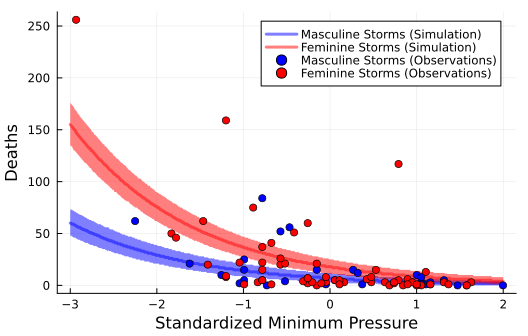
\includegraphics[keepaspectratio]{hw02_files/mediabag/hw02_files/figure-pdf/fig-hurricane-sim-output-1.pdf}}

}

\caption{\label{fig-hurricane-sim}Simulation of hurricane deaths based
on femininity of name and minimum hurricane pressure. Included are
projections assuming the most masculine and feminine names in the
dataset.}

\end{figure}%

The model fails to predict the storms with the most and least deaths for
both genders; this isn't entirely shocking since most of the data
consists of storms with low deaths, and a Poisson model has equal
variance to its mean. We would need a model with more dispersion (such
as a negative binomial, which was used in the original paper) to
potentially predict these. However, the model does clearly predict an
effect from the gender of the storm name, as we can see in
Figure~\ref{fig-hurricane-sim}.

\paragraph{Problem 4.3}\label{problem-4.3}

The effect size shown in Figure~\ref{fig-hurricane-sim} is quite strong,
and does not in general seem supported by the data. While there are
female-named storms with more deaths than the male-named storms with
similar minimum pressures, we can also see many cases where they are
quite similar. This effect seems to be driven by the large outlying
storms, which tend to have female names, but aside from these few
events, the data do not appear to suggest a systematic pattern of
greater deaths from female storms.

\paragraph{Problem 4.4}\label{problem-4.4}

We can now stop taking this hypothesis seriously. To what extent do you
think the finding could be an artifact of the dataset (e.g.~there is no
actual effect, but there are coincidental features of the data that
produce the result that female-named storms are more deadly than
male-named storms)? Justify this conclusion with specific reference to
an exploratory analysis of the data.

As noted in the solution to Problem 4.3, the model results seem to be
driven entirely by the most deadly four storms, all of which had female
names. We can see how likely this is from random variation. Let's look
at how many more storms in the dataset have female names than male
names.

\begin{Shaded}
\begin{Highlighting}[]
\FunctionTok{sum}\NormalTok{(dat.female) }\OperatorTok{/} \FunctionTok{nrow}\NormalTok{(dat)}
\end{Highlighting}
\end{Shaded}

\begin{verbatim}
0.6739130434782609
\end{verbatim}

So 2/3 of the storms in the dataset have female names. As a result,
there is a \((2/3)^4 =20\%\) probability that the four deadliest storms
would happen to have female names just by chance, which is hardly
negligible.

\textbf{Extra} (I don't expect you to have looked this up):

In fact, this isn't random: the dataset includes storms between
1953--1978, when all tropical storms were given female names. And in
fact, other than Sandy (which is classified as having a female name, but
it is generally considered unisex), the four most deadly storms were
from this period:

\begin{Shaded}
\begin{Highlighting}[]
\FunctionTok{sort}\NormalTok{(dat, }\OperatorTok{:}\NormalTok{deaths, rev}\OperatorTok{=}\ConstantTok{true}\NormalTok{)}
\end{Highlighting}
\end{Shaded}

\begin{tabular}{r|cccccccc}
    & name & year & deaths & category & min\_pressure & damage\_norm & female & femininity\\
    \hline
    & String15 & Int64 & Int64 & Int64 & Int64 & Int64 & Int64 & Float64\\
    \hline
    1 & Camille & 1969 & 256 & 5 & 909 & 23040 & 1 & 9.05556 \\
    2 & Diane & 1955 & 200 & 1 & 987 & 14730 & 1 & 9.88889 \\
    3 & Sandy & 2012 & 159 & 2 & 942 & 75000 & 1 & 9.0 \\
    4 & Agnes & 1972 & 117 & 1 & 980 & 20430 & 1 & 8.66667 \\
    5 & Ike & 2008 & 84 & 2 & 950 & 20370 & 0 & 1.88889 \\
    6 & Betsy & 1965 & 75 & 3 & 948 & 20000 & 1 & 8.33333 \\
    7 & Andrew & 1992 & 62 & 5 & 922 & 66730 & 0 & 2.22222 \\
    8 & Rita & 2005 & 62 & 3 & 937 & 10690 & 1 & 9.5 \\
    9 & Carol & 1954 & 60 & 3 & 960 & 19321 & 1 & 8.11111 \\
    10 & Floyd & 1999 & 56 & 2 & 956 & 8130 & 0 & 1.83333 \\
    11 & Gustav & 2008 & 52 & 2 & 954 & 4360 & 0 & 1.72222 \\
    12 & Isabel & 2003 & 51 & 2 & 957 & 4980 & 1 & 9.38889 \\
    13 & Donna & 1960 & 50 & 4 & 930 & 53270 & 1 & 9.27778 \\
    14 & Carla & 1961 & 46 & 4 & 931 & 15850 & 1 & 9.5 \\
    15 & Irene & 2011 & 41 & 1 & 952 & 7110 & 1 & 9.27778 \\
    16 & Hilda & 1964 & 37 & 3 & 950 & 2770 & 1 & 8.83333 \\
    17 & Fran & 1996 & 26 & 3 & 954 & 8260 & 1 & 7.16667 \\
    18 & Ivan & 2004 & 25 & 3 & 946 & 18590 & 0 & 1.05556 \\
    19 & Gracie & 1959 & 22 & 3 & 950 & 510 & 1 & 9.77778 \\
    20 & Celia & 1970 & 22 & 3 & 945 & 6870 & 1 & 9.44444 \\
    21 & Eloise & 1975 & 21 & 3 & 955 & 6190 & 1 & 8.94444 \\
    22 & Alicia & 1983 & 21 & 3 & 962 & 10400 & 1 & 9.83333 \\
    23 & Hugo & 1989 & 21 & 4 & 934 & 20020 & 0 & 2.88889 \\
    24 & Edna & 1954 & 20 & 3 & 954 & 3230 & 1 & 8.55556 \\
    $\dots$ & $\dots$ & $\dots$ & $\dots$ & $\dots$ & $\dots$ & $\dots$ & $\dots$ & $\dots$ \\
\end{tabular}

As noted, while Katrina and Audrey would have also been among the top
storms (but were left out of the dataset), Hurricane Audrey was in 1957,
which is also in the female-only period. Neglecting the storms from that
period makes the deadliest storms Katrina, Sandy, and Ike: hardly signs
of a clear female bias. Moreover, we know that many of the deaths from
Katrina resulted from engineering failures rather than residents ``not
taking storms with female names seriously.''

For a thorough analysis of this paper's statistical failings (which go
beyond what we have considered here), see
\href{https://www.sciencedirect.com/science/article/pii/S2212094715300517}{this
paper by Gary Smith}. As a sign of how much of a laughingstock this
paper is among statisticians, you can see how often it's mockingly
referenced at
\href{https://statmodeling.stat.columbia.edu/?s=himmicanes&submit=Search}{Andrew
Gelman's blog}. This is further evidence that just because you can do
statistics, it doesn't mean your results make sense, even if you fit
your model and get ``statistically significant'' results. You should
always think carefully about what your data-generating mechanism
actually implies, and how fit for purpose your dataset is to examine
your hypothesis (in this case, the inclusion of data between 1953 and
1978 clearly biases the results in favor of the authors' hypothesis).

\subsection{References}\label{references}




\end{document}
